% Options for packages loaded elsewhere
\PassOptionsToPackage{unicode}{hyperref}
\PassOptionsToPackage{hyphens}{url}
\PassOptionsToPackage{dvipsnames,svgnames,x11names}{xcolor}
%
\documentclass[
  letterpaper,
  DIV=11,
  numbers=noendperiod]{scrartcl}

\usepackage{amsmath,amssymb}
\usepackage{iftex}
\ifPDFTeX
  \usepackage[T1]{fontenc}
  \usepackage[utf8]{inputenc}
  \usepackage{textcomp} % provide euro and other symbols
\else % if luatex or xetex
  \usepackage{unicode-math}
  \defaultfontfeatures{Scale=MatchLowercase}
  \defaultfontfeatures[\rmfamily]{Ligatures=TeX,Scale=1}
\fi
\usepackage{lmodern}
\ifPDFTeX\else  
    % xetex/luatex font selection
\fi
% Use upquote if available, for straight quotes in verbatim environments
\IfFileExists{upquote.sty}{\usepackage{upquote}}{}
\IfFileExists{microtype.sty}{% use microtype if available
  \usepackage[]{microtype}
  \UseMicrotypeSet[protrusion]{basicmath} % disable protrusion for tt fonts
}{}
\makeatletter
\@ifundefined{KOMAClassName}{% if non-KOMA class
  \IfFileExists{parskip.sty}{%
    \usepackage{parskip}
  }{% else
    \setlength{\parindent}{0pt}
    \setlength{\parskip}{6pt plus 2pt minus 1pt}}
}{% if KOMA class
  \KOMAoptions{parskip=half}}
\makeatother
\usepackage{xcolor}
\setlength{\emergencystretch}{3em} % prevent overfull lines
\setcounter{secnumdepth}{4}
% Make \paragraph and \subparagraph free-standing
\makeatletter
\ifx\paragraph\undefined\else
  \let\oldparagraph\paragraph
  \renewcommand{\paragraph}{
    \@ifstar
      \xxxParagraphStar
      \xxxParagraphNoStar
  }
  \newcommand{\xxxParagraphStar}[1]{\oldparagraph*{#1}\mbox{}}
  \newcommand{\xxxParagraphNoStar}[1]{\oldparagraph{#1}\mbox{}}
\fi
\ifx\subparagraph\undefined\else
  \let\oldsubparagraph\subparagraph
  \renewcommand{\subparagraph}{
    \@ifstar
      \xxxSubParagraphStar
      \xxxSubParagraphNoStar
  }
  \newcommand{\xxxSubParagraphStar}[1]{\oldsubparagraph*{#1}\mbox{}}
  \newcommand{\xxxSubParagraphNoStar}[1]{\oldsubparagraph{#1}\mbox{}}
\fi
\makeatother

\usepackage{color}
\usepackage{fancyvrb}
\newcommand{\VerbBar}{|}
\newcommand{\VERB}{\Verb[commandchars=\\\{\}]}
\DefineVerbatimEnvironment{Highlighting}{Verbatim}{commandchars=\\\{\}}
% Add ',fontsize=\small' for more characters per line
\newenvironment{Shaded}{}{}
\newcommand{\AlertTok}[1]{\textcolor[rgb]{0.58,0.85,0.30}{\textbf{\colorbox[rgb]{0.30,0.12,0.14}{#1}}}}
\newcommand{\AnnotationTok}[1]{\textcolor[rgb]{0.31,0.63,0.31}{#1}}
\newcommand{\AttributeTok}[1]{\textcolor[rgb]{0.65,0.15,0.64}{#1}}
\newcommand{\BaseNTok}[1]{\textcolor[rgb]{0.60,0.41,0.00}{#1}}
\newcommand{\BuiltInTok}[1]{\textcolor[rgb]{0.65,0.15,0.64}{#1}}
\newcommand{\CharTok}[1]{\textcolor[rgb]{0.31,0.63,0.31}{#1}}
\newcommand{\CommentTok}[1]{\textcolor[rgb]{0.63,0.63,0.65}{\textit{#1}}}
\newcommand{\CommentVarTok}[1]{\textcolor[rgb]{0.89,0.34,0.29}{\textit{#1}}}
\newcommand{\ConstantTok}[1]{\textcolor[rgb]{0.60,0.41,0.00}{#1}}
\newcommand{\ControlFlowTok}[1]{\textcolor[rgb]{0.65,0.15,0.64}{#1}}
\newcommand{\DataTypeTok}[1]{\textcolor[rgb]{0.65,0.15,0.64}{#1}}
\newcommand{\DecValTok}[1]{\textcolor[rgb]{0.60,0.41,0.00}{#1}}
\newcommand{\DocumentationTok}[1]{\textcolor[rgb]{0.89,0.34,0.29}{#1}}
\newcommand{\ErrorTok}[1]{\textcolor[rgb]{0.96,0.28,0.28}{\underline{#1}}}
\newcommand{\ExtensionTok}[1]{\textcolor[rgb]{0.25,0.47,0.95}{\textbf{#1}}}
\newcommand{\FloatTok}[1]{\textcolor[rgb]{0.60,0.41,0.00}{#1}}
\newcommand{\FunctionTok}[1]{\textcolor[rgb]{0.25,0.47,0.95}{#1}}
\newcommand{\ImportTok}[1]{\textcolor[rgb]{0.31,0.63,0.31}{#1}}
\newcommand{\InformationTok}[1]{\textcolor[rgb]{0.77,0.36,0.00}{#1}}
\newcommand{\KeywordTok}[1]{\textcolor[rgb]{0.65,0.15,0.64}{#1}}
\newcommand{\NormalTok}[1]{\textcolor[rgb]{0.22,0.23,0.26}{#1}}
\newcommand{\OperatorTok}[1]{\textcolor[rgb]{0.65,0.15,0.64}{#1}}
\newcommand{\OtherTok}[1]{\textcolor[rgb]{0.15,0.68,0.38}{#1}}
\newcommand{\PreprocessorTok}[1]{\textcolor[rgb]{0.65,0.15,0.64}{#1}}
\newcommand{\RegionMarkerTok}[1]{\textcolor[rgb]{0.16,0.50,0.73}{\colorbox[rgb]{0.08,0.19,0.26}{#1}}}
\newcommand{\SpecialCharTok}[1]{\textcolor[rgb]{0.00,0.52,0.74}{#1}}
\newcommand{\SpecialStringTok}[1]{\textcolor[rgb]{0.85,0.27,0.33}{#1}}
\newcommand{\StringTok}[1]{\textcolor[rgb]{0.31,0.63,0.31}{#1}}
\newcommand{\VariableTok}[1]{\textcolor[rgb]{0.89,0.34,0.29}{#1}}
\newcommand{\VerbatimStringTok}[1]{\textcolor[rgb]{0.85,0.27,0.33}{#1}}
\newcommand{\WarningTok}[1]{\textcolor[rgb]{0.85,0.27,0.33}{#1}}

\providecommand{\tightlist}{%
  \setlength{\itemsep}{0pt}\setlength{\parskip}{0pt}}\usepackage{longtable,booktabs,array}
\usepackage{calc} % for calculating minipage widths
% Correct order of tables after \paragraph or \subparagraph
\usepackage{etoolbox}
\makeatletter
\patchcmd\longtable{\par}{\if@noskipsec\mbox{}\fi\par}{}{}
\makeatother
% Allow footnotes in longtable head/foot
\IfFileExists{footnotehyper.sty}{\usepackage{footnotehyper}}{\usepackage{footnote}}
\makesavenoteenv{longtable}
\usepackage{graphicx}
\makeatletter
\def\maxwidth{\ifdim\Gin@nat@width>\linewidth\linewidth\else\Gin@nat@width\fi}
\def\maxheight{\ifdim\Gin@nat@height>\textheight\textheight\else\Gin@nat@height\fi}
\makeatother
% Scale images if necessary, so that they will not overflow the page
% margins by default, and it is still possible to overwrite the defaults
% using explicit options in \includegraphics[width, height, ...]{}
\setkeys{Gin}{width=\maxwidth,height=\maxheight,keepaspectratio}
% Set default figure placement to htbp
\makeatletter
\def\fps@figure{htbp}
\makeatother
% definitions for citeproc citations
\NewDocumentCommand\citeproctext{}{}
\NewDocumentCommand\citeproc{mm}{%
  \begingroup\def\citeproctext{#2}\cite{#1}\endgroup}
\makeatletter
 % allow citations to break across lines
 \let\@cite@ofmt\@firstofone
 % avoid brackets around text for \cite:
 \def\@biblabel#1{}
 \def\@cite#1#2{{#1\if@tempswa , #2\fi}}
\makeatother
\newlength{\cslhangindent}
\setlength{\cslhangindent}{1.5em}
\newlength{\csllabelwidth}
\setlength{\csllabelwidth}{3em}
\newenvironment{CSLReferences}[2] % #1 hanging-indent, #2 entry-spacing
 {\begin{list}{}{%
  \setlength{\itemindent}{0pt}
  \setlength{\leftmargin}{0pt}
  \setlength{\parsep}{0pt}
  % turn on hanging indent if param 1 is 1
  \ifodd #1
   \setlength{\leftmargin}{\cslhangindent}
   \setlength{\itemindent}{-1\cslhangindent}
  \fi
  % set entry spacing
  \setlength{\itemsep}{#2\baselineskip}}}
 {\end{list}}
\usepackage{calc}
\newcommand{\CSLBlock}[1]{\hfill\break\parbox[t]{\linewidth}{\strut\ignorespaces#1\strut}}
\newcommand{\CSLLeftMargin}[1]{\parbox[t]{\csllabelwidth}{\strut#1\strut}}
\newcommand{\CSLRightInline}[1]{\parbox[t]{\linewidth - \csllabelwidth}{\strut#1\strut}}
\newcommand{\CSLIndent}[1]{\hspace{\cslhangindent}#1}

\usepackage{booktabs}
\usepackage{longtable}
\usepackage{array}
\usepackage{multirow}
\usepackage{wrapfig}
\usepackage{float}
\usepackage{colortbl}
\usepackage{pdflscape}
\usepackage{tabu}
\usepackage{threeparttable}
\usepackage{threeparttablex}
\usepackage[normalem]{ulem}
\usepackage{makecell}
\usepackage{xcolor}
\KOMAoption{captions}{tableheading}
\makeatletter
\@ifpackageloaded{caption}{}{\usepackage{caption}}
\AtBeginDocument{%
\ifdefined\contentsname
  \renewcommand*\contentsname{Table of contents}
\else
  \newcommand\contentsname{Table of contents}
\fi
\ifdefined\listfigurename
  \renewcommand*\listfigurename{List of Figures}
\else
  \newcommand\listfigurename{List of Figures}
\fi
\ifdefined\listtablename
  \renewcommand*\listtablename{List of Tables}
\else
  \newcommand\listtablename{List of Tables}
\fi
\ifdefined\figurename
  \renewcommand*\figurename{Figure}
\else
  \newcommand\figurename{Figure}
\fi
\ifdefined\tablename
  \renewcommand*\tablename{Table}
\else
  \newcommand\tablename{Table}
\fi
}
\@ifpackageloaded{float}{}{\usepackage{float}}
\floatstyle{ruled}
\@ifundefined{c@chapter}{\newfloat{codelisting}{h}{lop}}{\newfloat{codelisting}{h}{lop}[chapter]}
\floatname{codelisting}{Listing}
\newcommand*\listoflistings{\listof{codelisting}{List of Listings}}
\makeatother
\makeatletter
\makeatother
\makeatletter
\@ifpackageloaded{caption}{}{\usepackage{caption}}
\@ifpackageloaded{subcaption}{}{\usepackage{subcaption}}
\makeatother
\makeatletter
\@ifpackageloaded{tcolorbox}{}{\usepackage[skins,breakable]{tcolorbox}}
\makeatother
\makeatletter
\@ifundefined{shadecolor}{\definecolor{shadecolor}{named}{white}}{}
\makeatother
\makeatletter
\@ifundefined{codebgcolor}{\definecolor{codebgcolor}{HTML}{f8f8f8}}{}
\makeatother
\makeatletter
\ifdefined\Shaded\renewenvironment{Shaded}{\begin{tcolorbox}[colback={codebgcolor}, boxrule=0pt, frame hidden, breakable, borderline west={3pt}{0pt}{shadecolor}, enhanced, sharp corners]}{\end{tcolorbox}}\fi
\makeatother
\ifLuaTeX
  \usepackage{selnolig}  % disable illegal ligatures
\fi
\usepackage{bookmark}

\IfFileExists{xurl.sty}{\usepackage{xurl}}{} % add URL line breaks if available
\urlstyle{same} % disable monospaced font for URLs
\hypersetup{
  pdftitle={Quarto Markdown Template},
  pdfauthor={Yingqi Jing},
  colorlinks=true,
  linkcolor={blue},
  filecolor={Maroon},
  citecolor={Blue},
  urlcolor={Blue},
  pdfcreator={LaTeX via pandoc}}

\title{Quarto Markdown Template}
\author{Yingqi Jing}
\date{June 18, 2024}

\begin{document}
\maketitle

\renewcommand*\contentsname{Contents}
{
\hypersetup{linkcolor=}
\setcounter{tocdepth}{4}
\tableofcontents
}
\listoffigures
\listoftables
\clearpage

\section{Introduction}\label{introduction}

For large files, we can cache the file, and use
\texttt{cache.lazy\ =\ T} to reuse the pre-computed results. To avoid
overwriting the previously cached file, it is better to set the
\texttt{cache=\ F}, when you want to use cachy.lazy to get the
previously saved results. In this case, you do not need to cache the
file again. You can also load the cached file, and check the environment
to see whether the variables have already been saved.

If \texttt{cache\ =\ T}, knitr~will skip the execution of this code
chunk if it has been executed before and nothing in the code chunk has
changed since then. This is particularly useful when you want to reuse
the figure (time-consuming). \textbf{When you modify the code chunk
(e.g., revise the code or the chunk options), the previous cache will be
automatically invalidated, and knitr will cache the chunk again.}

You can also use cross-reference for a Section~\ref{sec-data-method}.

You can also cite a paper like this (\citeproc{ref-Kirby2016}{Kirby et
al. 2016}).

\begin{Shaded}
\begin{Highlighting}[]
\FunctionTok{print}\NormalTok{(}\StringTok{"Hello R markdown!"}\NormalTok{)}
\end{Highlighting}
\end{Shaded}

\begin{verbatim}
[1] "Hello R markdown!"
\end{verbatim}

\begin{Shaded}
\begin{Highlighting}[]
\FunctionTok{ls}\NormalTok{ figures/}\PreprocessorTok{*}
\end{Highlighting}
\end{Shaded}

\begin{verbatim}
figures/CTMCgraphs-1.pdf
figures/CTMCgraphs-1.png
figures/fig-histogram-rng-1.png
figures/histogram-1.png
figures/histogram-rng-1.png
figures/simpletikz 2-1.png
figures/simpletikz-1.pdf
figures/simpletikz-1.png
figures/simpletikz2-1.pdf
\end{verbatim}

\section{Data and Methods}\label{sec-data-method}

\begin{tabular}{|l|l|}\hline
Age & Frequency \\ \hline
18--25  & 15 \\
26--35  & 33 \\
36--45  & 22 \\ \hline
\end{tabular}

\begin{Shaded}
\begin{Highlighting}[]
\PreprocessorTok{\#include }\ImportTok{\textless{}Rcpp.h\textgreater{}}
\KeywordTok{using} \KeywordTok{namespace}\NormalTok{ Rcpp}\OperatorTok{;}
\CommentTok{// [[Rcpp::export]]}
\NormalTok{NumericVector timesTwo}\OperatorTok{(}\NormalTok{NumericVector x}\OperatorTok{)} \OperatorTok{\{}
  \ControlFlowTok{return}\NormalTok{ x }\OperatorTok{*} \DecValTok{2}\OperatorTok{;}
\OperatorTok{\}}
\end{Highlighting}
\end{Shaded}

\begin{Shaded}
\begin{Highlighting}[]
\FunctionTok{timesTwo}\NormalTok{(}\DecValTok{10}\NormalTok{) }\CommentTok{\# test function in R chunk or console}
\end{Highlighting}
\end{Shaded}

\section{Results}\label{results}

We can also save the plot as png files, by setting the dev = ``png'',
and change the quality of the picture by setting dpi = 300.

Alternatively, you can convert all the saved pdfs into pngs with
imagemagick in terminal:

\begin{Shaded}
\begin{Highlighting}[]
\ExtensionTok{convert} \AttributeTok{{-}density}\NormalTok{ 150 }\PreprocessorTok{*}\NormalTok{.pdf }\AttributeTok{{-}quality}\NormalTok{ 100 }\AttributeTok{{-}set}\NormalTok{ filename:basename }\StringTok{"\%[basename]"} \StringTok{"\%[filename:basename].png"}
\end{Highlighting}
\end{Shaded}

\subsection{Cross-reference of figures, tables and
equations}\label{cross-reference-of-figures-tables-and-equations}

In order to decrease the figure sizes, you can try to use png or jpeg
rather than pdf output.

\begin{figure}

\centering{

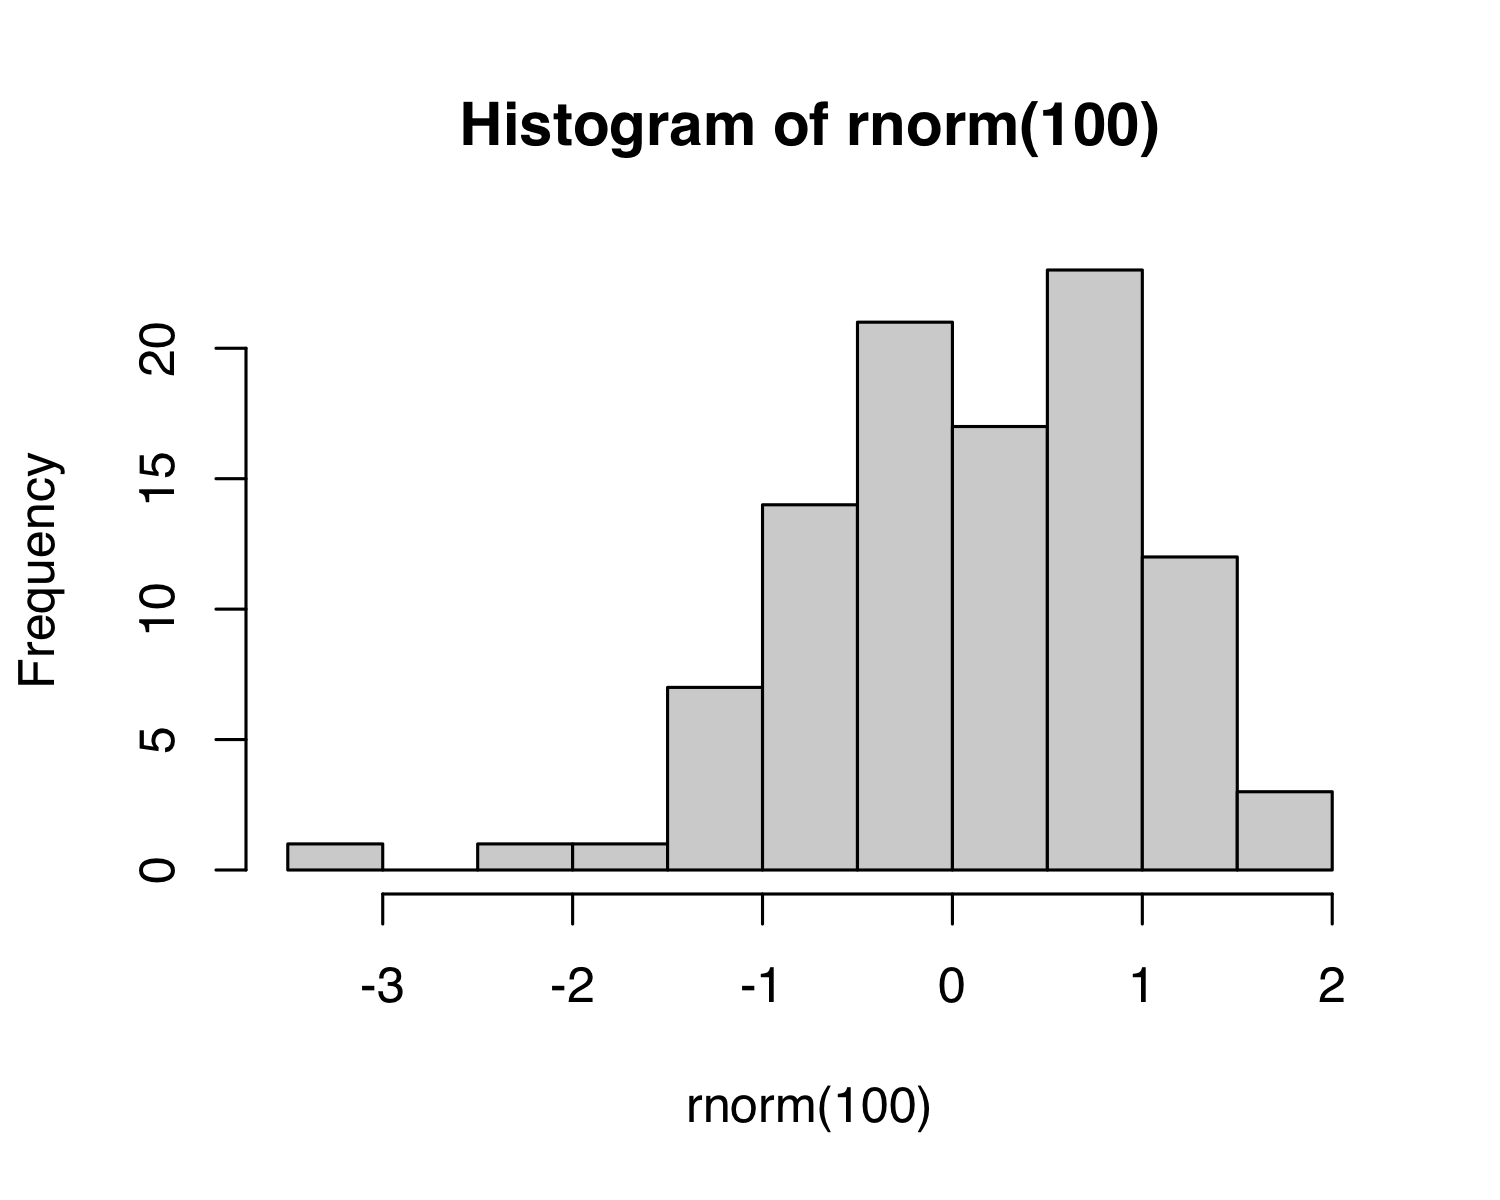
\includegraphics{figures/fig-histogram-rng-1.png}

}

\caption{\label{fig-histogram-rng}Histogram plot}

\end{figure}%

We can also co-refer a plot in Figure~\ref{fig-histogram-rng}.
\textbf{Note:} you need to set \texttt{include\ =\ T} when producing the
plot. Otherwise, the co-reference won't work.

\begin{Shaded}
\begin{Highlighting}[]
\CommentTok{\# two ways of include a picture in R}
\CommentTok{\# ![example picture](./figures/histogram{-}1.png)\{width=90\% height=80\%\}}
\NormalTok{knitr}\SpecialCharTok{::}\FunctionTok{include\_graphics}\NormalTok{(}\StringTok{"./figures/histogram{-}rng{-}1.png"}\NormalTok{)}
\end{Highlighting}
\end{Shaded}

\subsection{Citations}\label{citations}

You can cite a paper in Rmarkdown in different ways, e.g., if you want
to have the citation with exact page number. You can use the following
ways (see \citeproc{ref-Jing2022}{Jing et al. 2022:45}) or Jing et al.
(\citeproc{ref-Jing2022}{2022:404}).

\section{Discussion}\label{discussion}

\begin{figure}[H]

{\centering 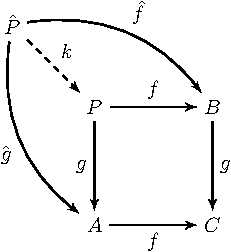
\includegraphics{figures/simpletikz-1.pdf}

}

\caption{Tikz graph example}

\end{figure}%

\section{Conclusions}\label{conclusions}

\textbf{Note:} it seems that tikz does not support both fig.cap and
fig.scap at the same time. It may cause fig.cap cannot recognize the
latex code.

We can also add the cross-reference inside the figure cation via
\texttt{\textbackslash{}\textbackslash{}ref\{fig:\}}.

\clearpage

\section*{References}\label{references}
\addcontentsline{toc}{section}{References}

\phantomsection\label{refs}
\begin{CSLReferences}{1}{0}
\bibitem[\citeproctext]{ref-Jing2022}
Jing, Yingqi, Damián E Blasi \& Balthasar Bickel. 2022.
Dependency-Length Minimization and Its Limits: {A} Possible Role for a
Probabilistic Version of the Final-over-Final Condition. \emph{Language}
98(3). 397--418.
doi:\href{https://doi.org/10.1353/lan.0.0267}{10.1353/lan.0.0267}.

\bibitem[\citeproctext]{ref-Kirby2016}
Kirby, Kathryn R., Russell D. Gray, Simon J. Greenhill, Fiona M. Jordan,
Stephanie Gomes-Ng, Hans-Jörg Bibiko, Damián E. Blasi, Carlos A. Botero,
Claire Bowern, Carol R. Ember, et al. 2016. D-{PLACE}: {A Global
Database} of {Cultural}, {Linguistic} and {Environmental Diversity}.
\emph{PLOS ONE} 11(7). e0158391.
doi:\href{https://doi.org/10.1371/journal.pone.0158391}{10.1371/journal.pone.0158391}.

\end{CSLReferences}



\end{document}
